\documentclass[../main.tex]{subfiles}
\begin{document}
\chapter{AFM - SNOM}
Le immagini prese in esame in questa tesi sono state prodotte con un microscopio NeaSNOM. In questo capitolo viene descritta la sua struttura e le sue modalità di funzionamento...
\change{Imposta una introduzione quando finisci il capitolo}
\section{Storia della Microscopia}

I primi microscopi composti costruiti risalgono al 17\textdegree\ secolo, oltre 400 anni fa. È in quest'epoca che si riuscì a vedere per la prima volta i microrganismi che abitano la Terra ed ebbe inizio lo studio della \gls{microbiologia}. \textit{Robert Hooke} osservò le pareti cellulari e usò per la prima volta il termine ``cellula" \cite{fara_2009, micrographia}, mentre \textit{Antoine van Leeuwenhoek} sviluppò dei microscopi semplici (a singola lente) con ingrandimenti molto superiori a quelli degli strumenti contemporanei e fu il primo ad osservare microrganismi, come batteri e globuli rossi.\cite{lane_2015, dobell_1923, corliss_1975, jessup_2024}

\subsection{Microscopio ottico composto}

Il microscopio ottico composto ingrandisce l'immagine del campione usando delle lenti. il campione può essere illuminato facendolo attraversare dalla luce sul lato opposto all'obiettivo (microscopia a luce trasmessa) oppure riflettendocela sopra (microscopia a luce riflessa).

Il sistema più semplice è composto da due lenti, una lente obiettivo vicina al campione da esaminare, e una lente oculare vicina all'osservatore. Il campione è prima messo a fuoco dalla lente obiettivo dentro al microscopio in una immagine reale, poiché è creata dalla convergenza dei raggi di luce, poi questa immagine viene nuovamente ingrandita dalla lente oculare che crea una nuova immagine, stavolta virtuale visto che è creata da proiezioni di raggi divergenti. L'osservatore quindi vedrà un'immagine ingrandita, invertita e virtuale del campione esaminato.

\begin{figure}[h]
\centering
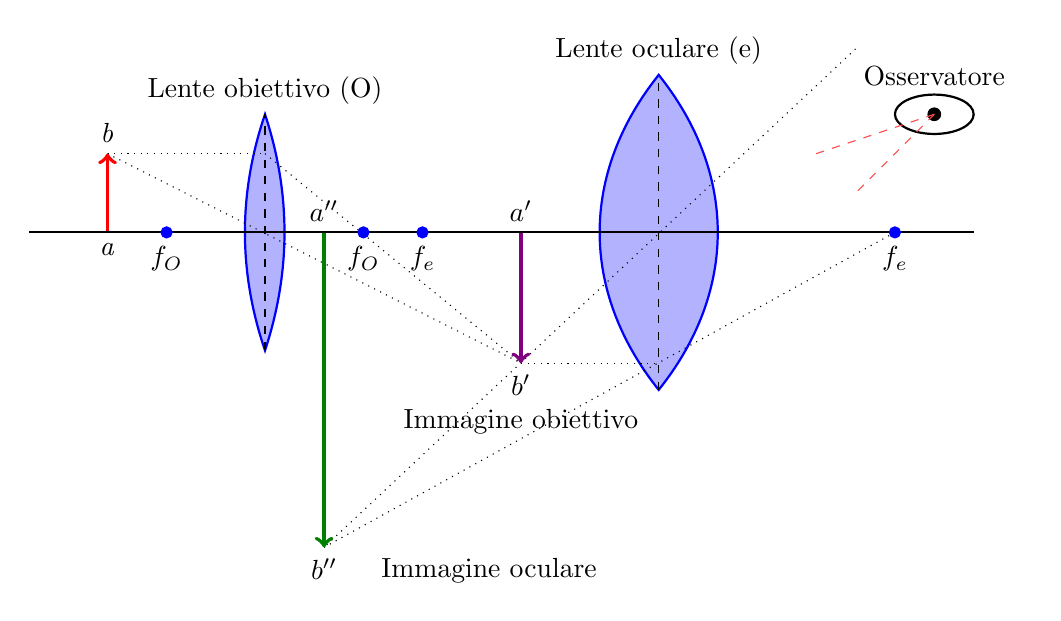
\begin{tikzpicture}
	% lente obiettivo
	\filldraw[thick,blue!30, draw=blue] (3,1.5)
		.. controls (2.66,0.5) and (2.66,-0.5) .. (3,-1.5)
		.. controls (3.33,-0.5) and (3.33,0.5) .. cycle
		node[black,above] {Lente obiettivo (O)};
	\draw[dashed] (3,-1.5) -- (3,1.5);

	% lente oculare
	\filldraw[thick,blue!30, draw=blue] (8,2)
	.. controls (9,0.75) and (9,-0.75) .. (8,-2)
	.. controls (7,-0.75) and (7,0.75) .. cycle
	node[black,above] {Lente oculare (e)};
	\draw[dashed] (8,-2) -- (8,2);

	\draw[dotted] (1,1) -- (3,1);
	\draw[dotted] (3,1) -- (6.25,-1.66);
	\draw[dotted] (1,1) -- (6.25,-1.66);

	\draw[dotted] (6.25,-1.66) -- (8,-1.66);
	\draw[dotted] (11,0) -- (3.75,-4);
	\draw[dotted] (10.5,2.33) -- (3.75,-4);

	% oggetto
	\draw[line width=0.5mm,Red,->] (1,0) node[below, black] {\textit{a}}
		-- (1,1) node[above, black] {\textit{b}};

	% immagine reale
	\draw[line width=0.5mm,Purple,->] (6.25,0) node[above, black] {$a'$}
		-- (6.25,-1.66) node[below, black, align=center] {$b'$ \\ \text{Immagine obiettivo}};

	% immagine virtuale
	\draw[line width=0.5mm,Green,->] (3.75,0) node[above, black] {$a''$}
		-- (3.75,-4) node[below, black] {$b''$} node[below right, black] {\ \ \quad Immagine oculare};

	% linea principale
	\draw[thick] (0,0) -- (12,0);

	% lunghezza focale lente oculare
	\filldraw[blue] (5,0) circle (2pt) node[below,black,inner sep=5pt]{$f_e$};
	\filldraw[blue] (11,0) circle (2pt) node[below,black,inner sep=5pt]{$f_e$};

	% lunghezza focale lente obiettivo
	\filldraw[blue] (1.75,0) circle (2pt) node[below,black,inner sep=5pt]{$f_O$};
	\filldraw[blue] (4.25,0) circle (2pt) node[below,black,inner sep=5pt]{$f_O$};

	% occhio
	\draw[thick] (11.5,1.5) ellipse (0.5 and 0.25)
		node[above, inner sep=10pt] {Osservatore};

	% pupilla
	\filldraw[black] (11.5,1.5) circle (0.08);

	% raggi visivi
	\draw[red!70, dashed] (11.5,1.5) -- (10,1);
	\draw[red!70, dashed] (11.5,1.5) -- (10.5,0.5);
\end{tikzpicture}
\caption{Principio di funzionamento di un microscopio ottico composto}
\label{fig:com_diag}
\end{figure}

Il microscopio ottico composto ha continuato ad essere sviluppato fino ad oggi e ne sono state create molte varianti per scopi più specializzati, come il microscopio a contrasto di fase (\acrshort{pcm})\cite{zernike_1955} o il microscopio confocale (\acrshort{clsm})\cite{pawley_2006}. In generale, oggi la microscopia ottica ha raggiunto altissimi livelli di prestazioni, sia ottiche che meccaniche, ma la cui risoluzione spaziale è rimasta bloccata dal limite di diffrazione della luce.

\subsection{Apertura numerica}

Il primo a definire questo limite fu \textit{Ernst Abbe} nel 1881, anno in cui pubblicò il suo lavoro sulla misura dell'apertura dei microscopi.\cite{abbe_1881} Questo limite, chiamato apertura numerica (\acrshort{na}), si basa sull'intervallo degli angoli con cui la luce può entrare o uscire dal microscopio  ed è comunemente usato in microscopia come parametro delle ottiche per valutarne la risoluzione. Questo numero è definito come il prodotto tra l'indice di rifrazione \textit{n} e il seno dell'apertura angolare della lente.

\begin{equation}
	\mathit{NA}=n\sin\theta
\end{equation}

Da questa formula, Abbe continuò il suo lavoro arrivando a definire anche la distanza minima tra due elementi diversi affinché si possano apprezzare attraverso un microscopio.\cite{abbe_1882}

\begin{equation}
d=\frac{\lambda}{2\mathit{NA}}=\frac{\lambda}{2n\sin\theta}
\end{equation}

Usando l'aria come mezzo di trasmissione si ha un indice di rifrazione di 1, mentre si può arrivare fino a circa 1.5 immergendo il campione e l'obiettivo in olio. Per quanto riguarda l'apertura angolare massima,  teoricamente può arrivare fino a 180\degree, il che si traduce in un valore di $\theta=90$\degree, ma ad ora le lenti con la più alta apertura angolare mai realizzate si fermano approssimativamente a 144\degree, che corrisponde a un valore di $\sin\left(\theta=72\degree\right) \approx 0.95$.\cite{leica_aperture}\\

\begin{figure}[h]
\centering
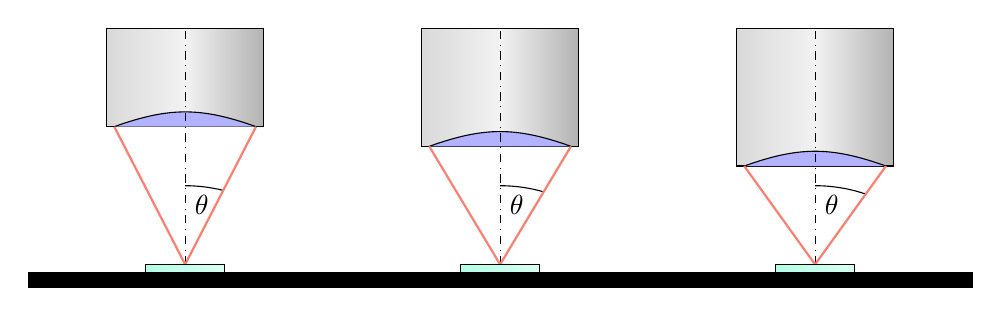
\begin{tikzpicture}
	%primo obiettivo
	\shadedraw[left color=gray!30, right color=gray!60, middle color=gray!10] (1,1.75) -- (1,3) -- (3,3) --(3,1.75) -- cycle;
	\filldraw[blue!30, draw=black] (1.1,1.75)
		.. controls (1.8,2) and (2.2,2)
		.. (2.9,1.75);
	\draw[dash dot] (2,0) -- (2,3);
	\draw (2,1) node[below right]{$\theta$} arc (90:76:2);
	\draw[Salmon, thick] (1.1,1.75) -- (2,0) -- (2.9,1.75);
	\shadedraw[left color=Aquamarine!60, right color=Aquamarine!30] (1.5,0) rectangle (2.5,-0.1);

	%secondo obiettivo
	\shadedraw[left color=gray!30, right color=gray!60, middle color=gray!10] (5,1.5) -- (5,3) -- (7,3) --(7,1.5) -- cycle;
	\filldraw[blue!30, draw=black] (5.1,1.5)
	.. controls (5.8,1.75) and (6.2,1.75)
	.. (6.9,1.5);
	\draw[dash dot] (6,0) -- (6,3);
	\draw (6,1) node[below right]{$\theta$} arc (90:74:2);
	\draw[Salmon, thick] (5.1,1.5) -- (6,0) -- (6.9,1.5);
	\shadedraw[left color=Aquamarine!60, right color=Aquamarine!30] (5.5,0) rectangle (6.5,-0.1);

	%terzo obiettivo
	\shadedraw[left color=gray!30, right color=gray!60, middle color=gray!10] (9,1.25) -- (9,3) -- (11,3) --(11,1.25) -- cycle;
	\filldraw[blue!30, draw=black] (9.1,1.25)
	.. controls (9.8,1.5) and (10.2,1.5)
	.. (10.9,1.25);
	\draw[dash dot] (10,0) -- (10,3);
	\draw (10,1) node[below right]{$\theta$} arc (90:71:2);
	\draw[Salmon, thick] (9.1,1.25) -- (10,0) -- (10.9,1.25);
	\shadedraw[left color=Aquamarine!60, right color=Aquamarine!30] (9.5,0) rectangle (10.5,-0.1);

	%base
	\fill[black] (0,-0.1) rectangle (12,-0.3);
\end{tikzpicture}
\caption{Obiettivi con diverse aperture}
\label{fig:na_diag}
\end{figure}

Per migliorare la risoluzione oltre il limite dei 250nm, ottenibili usando lunghezze d'onda dello spettro visibile, si possono scegliere onde elettromagnetiche a lunghezza minore, come i raggi X o UV, oppure raggi di altra natura, come i fasci di elettroni. Queste tecniche portano una risoluzione maggiore ma anche delle controindicazioni, come una scarsa risposta da parte del campione oppure tossicità.\cite{hell_2007}

\subsection{Microscopio elettronico}

La scoperta che i raggi di elettroni si comportano come onde con lunghezze d'onda più corte della luce visibile aprì nuove opportunità. I primi esemplari furono sviluppati nel 1931 da \textit{Max Knoll} e \textit{Ernst Ruska}\cite{oatley1982early} e già due anni dopo furono in grado di apprezzare dettagli oltre il limite dei microscopi ottici tradizionali.\cite{physics_nobel}

I microscopi elettronici utilizzano un fascio di elettroni al posto della luce e delle lenti magnetiche invece che ottiche. Usando raggi di elettroni invece che di luce, questi microscopi non misurano l'interazione tra materia e luce ma tra materia ed elettroni, aprendo le porte a nuovi campi di studio.

Nei primi microscopi elettronici, il campione da esaminare è posto tra il cannone elettronico e il rilevatore e l'immagine si forma in base a come gli elettroni vengono trasmessi attraverso il campione, che deve essere molto sottile (meno di 100nm). Questo tipo di microscopi si chiama microscopio elettronico \textit{a trasmissione} (\acrshort{tem}) e i modelli più recenti possono arrivare a risoluzioni spaziali fino a 0.5\AA\ (50pm).\cite{rolf_2009}

Un altro tipo molto usato di microscopi elettronici è quello \textit{a scansione} (\acrshort{sem}), in cui non si rileva il fascio trasmesso attraverso il campione bensì i raggi secondari che sono generati dalla loro interazione (come elettroni secondari o raggi X). Questa tecnica può ottenere immagini tridimensionali e non richiede un campione sottile quanto la \acrshort{tem}. Modelli recenti di \acrshort{sem} possono arrivare a risoluzioni spaziali fino a 0.4nm.\cite{hitachi_sem}\\

\begin{figure}[htbp]
\centering
\begin{subfigure}[t]{4.5cm}
	\centering
	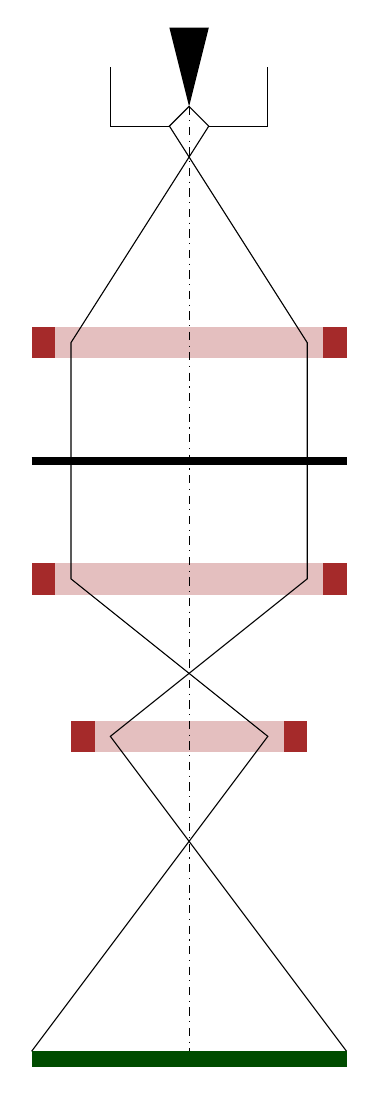
\begin{tikzpicture}
		%cannone
		\fill (1.75,1) -- (2,0) -- (2.25,1) -- cycle;
		\draw (1,0.5) -- (1,-0.25) -- (1.75,-0.25);
		\draw (3,0.5) -- (3,-0.25) -- (2.25,-0.25);

		% condensatore
		\fill[Brown] (0.3,-3.2) rectangle (0,-2.8);
		\fill[Brown] (3.7,-3.2) rectangle (4,-2.8);
		\fill[Brown!30] (0.3,-3.2) rectangle (3.7,-2.8);

		%obiettivo
		\fill[Brown] (0.3,-6.2) rectangle (0,-5.8);
		\fill[Brown] (3.7,-6.2) rectangle (4,-5.8);
		\fill[Brown!30] (0.3,-6.2) rectangle (3.7,-5.8);

		%proiettore
		\fill[Brown] (0.8,-8.2) rectangle (0.5,-7.8);
		\fill[Brown] (3.2,-8.2) rectangle (3.5,-7.8);
		\fill[Brown!30] (0.8,-8.2) rectangle (3.2,-7.8);

		\draw (2,0) -- (1.75,-0.25) -- (3.5,-3) -- (3.5,-6) -- (1,-8) -- (4,-12);
		\draw (2,0) -- (2.25,-0.25) -- (0.5,-3) -- (0.5,-6) -- (3,-8) -- (0,-12);

		\draw[line width=1mm] (0,-4.5) -- (4,-4.5);

		\draw[dash dot] (2,0) -- (2,-12);
		\fill[Green!60!Black] (0,-12) rectangle (4,-12.2);
	\end{tikzpicture}
	\caption{TEM}
\end{subfigure}
\hfill
\begin{minipage}[t]{0.3\textwidth}
	\centering
	\vspace{-12.4cm} Cannone elettronico\\
	\vspace{2.6cm} Lente condensatore\\
	\vspace{1.05cm} Campione\\
	\vspace{1.05cm} Lente obiettivo\\
	\vspace{0.525cm} Bobina di scansione\\
	\vspace{0.525cm} Lente proiettore\\
	\vspace{2cm} Campione\\
	\vspace{1.05cm} Camera CCD\\
\end{minipage}%
\begin{subfigure}[t]{5cm}
	\centering
	\begin{tikzpicture}
		%cannone
		\fill (1.75,1) -- (2,0) -- (2.25,1) -- cycle;
		\draw (1,0.5) -- (1,-0.25) -- (1.75,-0.25);
		\draw (3,0.5) -- (3,-0.25) -- (2.25,-0.25);

		% condensatore
		\fill[Brown] (0.3,-3.2) rectangle (0,-2.8);
		\fill[Brown] (3.7,-3.2) rectangle (4,-2.8);
		\fill[Brown!30] (0.3,-3.2) rectangle (3.7,-2.8);

		% deflettore
		\fill[Blue] (1.7,-6.2) rectangle (1.4,-5.8);
		\fill[Blue] (2.3,-6.2) rectangle (2.6,-5.8);
		\fill[Blue!30] (1.7,-6.2) rectangle (2.3,-5.8);

		%proiettore
		\fill[Brown] (0.8,-8.2) rectangle (0.5,-7.8);
		\fill[Brown] (3.2,-8.2) rectangle (3.5,-7.8);
		\fill[Brown!30] (0.8,-8.2) rectangle (3.2,-7.8);

		%campione
		\draw (2.5,-9.6) -- (1.2,-10) -- (2,-11.2) -- (3.3,-10.8) -- cycle;
		\coordinate (A) at (2.5,-9.6);
		\coordinate (B) at (1.2,-10);
		\coordinate (C) at (2,-11.2);
		\coordinate (D) at (3.3,-10.8);
		\foreach \t in {0.125,0.25,...,0.875} {
			\path
        		coordinate (L) at ($(B)!\t!(A)$)
				coordinate (R) at ($(C)!\t!(D)$);
			\draw[red, dashed, ->] (L) -- (R);
		};

		\draw (2,0) -- (1.75,-0.25) -- (3.5,-3) -- (1,-8) -- (2,-10);
		\draw (2,0) -- (2.25,-0.25) -- (0.5,-3) -- (3,-8) -- (2,-10);

		%indicazioni
		\draw (1.5,-6) -- (-0.5,-7.1);

		\draw[dash dot] (2,0) -- (2,-10);
		\fill[transparent] (0,-12.2){};
	\end{tikzpicture}
	\caption{SEM}
\end{subfigure}%
\caption{Principio di funzionamento dei microscopi TEM e SEM}
\label{fig:em_diag}
\end{figure}

Una limitazione di questi tipi di microscopi è che il campione deve essere conduttivo, altrimenti gli elettroni si accumulano sulla superficie del campione e lo caricano, distorcendo l'immagine. Per questo motivo, i campioni non conduttivi devono essere rivestiti con uno strato di metallo (come oro o carbonio) per permettere la conduzione degli elettroni.


\subsection{Microscopio a effetto tunnel}

La branca di microscopia di cui fa parte quello di interesse in questa tesi è lam microscopia a scansione di sonda (\acrshort{spm}) e fu fondata nel 1981 con l'invenzione del microscopio a effetto tunnel (\acrshort{stm}).\cite{ieee_spm}
Questi microscopi rilevano la superficie del campione usando una punta minuscola su cui è imposta una differenza di potenziale con il piano di osservazione. Mantenendo l'altezza della punta costante, si può misurare direttamente la variazione di corrente attraverso il campione in movimento, mentre per misurarne l'altezza si può mantenere costante la corrente e applicare un feedback al motore piezoelettrico che regola l'altezza della punta. Avendo una risoluzione di 0.1nm, questa tecnica permette di osservare singoli atomi, ma può essere usata solo se il campione è conduttivo.\cite{bai_2000}

\begin{figure}[h]
\centering
\begin{tikzpicture}
	% punta
	\filldraw[fill=gray] (-0.25,0) -- (-0.25,-1.75) -- (0,-2.5) -- (0.25,-1.75)
		node[right, xshift=3mm] {Punta}
		-- (0.25,0);

	% sistema di controllo
	\fill (-2.5,-1.9) rectangle (-2.45,-1.6);
	\fill (-2.4,-2.1) rectangle (-2.35,-1.4);
	\fill (-2.3,-1.9) rectangle (-2.25,-1.6);
	\fill (-2.2,-2.1) rectangle (-2.15,-1.4);
	\fill (-2.1,-1.9) rectangle (-2.05,-1.6);
	\fill (-2.0,-2.1) rectangle (-1.95,-1.4);
	\draw (-1.95,-1.75) node[above right] {\textbf{+}}
		-- (-0.25,-1.75);
	\draw (-2.5,-3.6) -- (-3,-3.6) -- (-3,-1.75) -- (-2.5,-1.75);
	\draw (-3,-2.75) -- (-5,-2.75) -- (-5, 0);
	\filldraw[fill=white] (-3,-2.75) circle (0.33)
		node[below left, xshift=-3mm, yshift=-3mm] {Amperometro};
	\draw[->] (-3.15,-2.9) -- (-2.85,-2.6);
	\draw[->] (-5,0) -- (-1,0);
	\node[draw, fill=white, align=center] at (-5,0) {Elettronica\\di controllo};

	% cilindro
	\node[cylinder, minimum height=2.5cm, minimum width=2cm, rotate=90, draw,
		shading=axis, left color=gray!30, right color=gray!60, middle color=gray!10] {};
	\filldraw[fill=white] (0,1.225) ellipse (1cm and 0.12cm)
		node[right, xshift=13mm] {Scanner};

	\draw[<->, thick] (1,1.5) -- (-1,1.5) node[midway, above] {X,Y};

	\draw (1,0)
		node[right, xshift=3mm] {Motore piezoelettrico}
		.. controls (1,-0.2) and (-1,-0.2) .. (-1,0);

	\draw[<->, thick] (0,-0.2) -- (0,-1.1) node[midway, right] {Z};

	% campione
	\filldraw[fill=purple] (-2,-3.5) -- (-2,-3.25)
		.. controls (-2,-3) and (-1.33,-3) .. (-1.25,-3.25)
		.. controls (-1,-3.3) and (-0.5, -2.9) .. (0.25,-3.25)
		.. controls (0.75,-3.4) and (1,-3.1) .. (1.7,-3.25)
		.. controls (1.8, -3.2) and (1.9, -3) .. (2,-3)
	 	-- (2,-3.5) node[above right, xshift=3mm] {Campione}
	 	-- cycle;

	 %base
	 \fill (-2.5,-3.5) rectangle (2.5,-3.7);

\end{tikzpicture}
\caption{Principio di funzionamento di un microscopio a effetto tunnel}
\label{fig:stm_di1ag}
\end{figure}

\section{AFM}

Una delle tecniche di microscopia che sono state usate per acquisire le immagini trattate in questa tesi è la microscopia a forza atomica (\acrshort{afm}). Questa tecnica è stata sviluppata nel 1986 da \textit{Gerd Binnig} e \textit{Heinrich Rohrer} ed è un altro tipo di tecnica di microscopia \acrshort{spm} che, permettendo di osservare campioni non conduttivi, a differenza della microscopia \acrshort{stm}, ha aperto la strada a nuove applicazioni.\cite{binnig_1986}

\subsection{Principio di funzionamento}

I microscopi \acrshort{afm} usano una punta di diametro di circa 10nm fissata a un braccio elastico (\textit{cantilever}), che viene fatta scorrere sulla superficie del campione. La dimensione della punta è importante perché influisce sulla risoluzione spaziale dell'immagine, che può arrivare anche a frazioni di nanometri. La fabbricazione di punte con un raggio così piccolo è uno dei limiti tecnici della microscopia \acrshort{afm} e il loro spessore minuscolo fa si che possano essere facilmente danneggiate.\\

\begin{figure}[H]
	\centering
	\begin{subfigure}{4cm}
		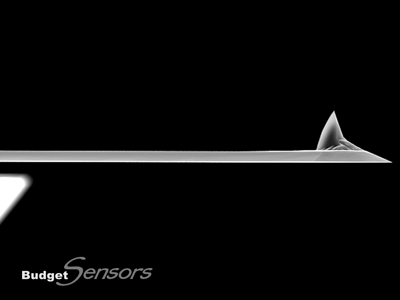
\includegraphics[width=4cm]{images/afm_tip.png}
		\caption{Vista laterale}
	\end{subfigure}
	\hfill
	\begin{subfigure}{4cm}
		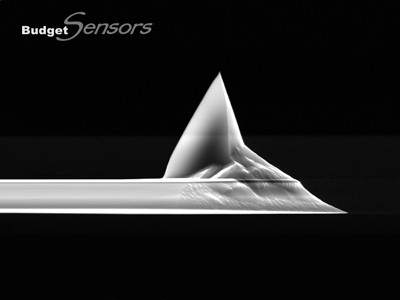
\includegraphics[width=4cm]{images/afm_tip_zoom.png}
		\caption{Vista ingrandita}
	\end{subfigure}
	\hfill
	\begin{subfigure}{4cm}
		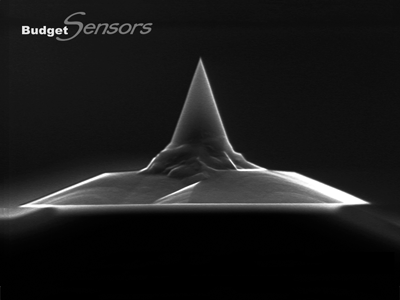
\includegraphics[width=4cm]{images/afm_tip_front.png}
		\caption{Vista frontale}
	\end{subfigure}
\caption{Punta di un microscopio \acrshort{afm} vista al microscopio \acrshort{sem}\ \cite{budgetsensors} }
\label{fig:afm_tip}
\end{figure}

Durante la scansione, la punta viene inclinata verso l'alto e il basso a causa della forza di interazione con il campione, che può essere di tipo repulsivo o attrattivo in base alla modalità di scansione. Queste inclinazioni vengono misurate da un raggio laser che viene riflesso dal cantilever su un fotodiodo a quadranti. L'inclinazione del cantilever deflette il raggio laser, che si sposta fra i quadranti del fotodiodo, e la variazione della corrente tra i quadranti viene poi convertita in una variazione di altezza della punta, che viene usata per generare l'immagine del campione.

Per effettuare la scansione, il piatto su cui poggia il campione viene spostato da degli elementi piezoelettrici, che possono espandersi e contrarsi con una precisione nanometrica variando una piccola tensione imposta (mV). Questi elementi piezoelettrici sono in grado di muoversi in tre direzioni (X, Y, Z) e sono controllati da un sistema elettronico che regola il movimento del campione in modo da mantenere il segnale di riferimento costante.

Con questo sistema si possono apprezzare variazioni di altezza fino a 0.01nm.\cite{sun_2018}

\begin{figure}[h]
\centering
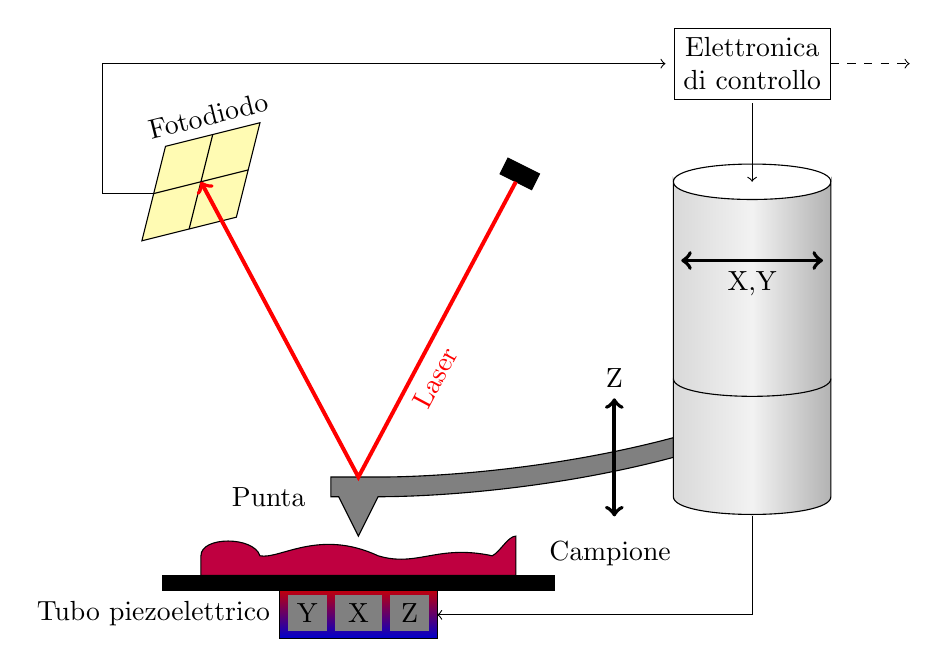
\begin{tikzpicture}
	% punta
	\filldraw[fill=gray] (0.25,-2.25) -- (-0.35,-2.25) -- (-0.35,-2.5)
		-- (-0.25,-2.5) node[left, xshift=-3mm] {Punta}
		-- (0,-3) -- (0.25,-2.5)
		.. controls (1,-2.5) and (2.5, -2.4) .. (4,-2)
		-- (4,-1.75)
		.. controls (2.5, -2.15) and (1,-2.25) .. cycle;

	% campione
	\filldraw[fill=purple] (-2,-3.5) -- (-2,-3.25)
		.. controls (-2,-3) and (-1.33,-3) .. (-1.25,-3.25)
		.. controls (-1,-3.3) and (-0.5, -2.9) .. (0.25,-3.25)
		.. controls (0.75,-3.4) and (1,-3.1) .. (1.7,-3.25)
		.. controls (1.8, -3.2) and (1.9, -3) .. (2,-3)
	 	-- (2,-3.5) node[above right, xshift=3mm] {Campione}
	 	-- cycle;

	%base
	\shadedraw[top color=red!80!black, bottom color=blue!80!black] (-1,-3.65)
		node[below left, yshift=-0.5mm] {Tubo piezoelettrico}
		rectangle (1,-4.3);

	\fill (-2.5,-3.5) rectangle (2.5,-3.7);

	\fill[color=gray] (0.4,-3.75) rectangle (0.9,-4.2) node[midway,black] {Z};
	\fill[color=gray] (-0.4,-3.75) rectangle (-0.9,-4.2) node[midway,black] {Y};
	\fill[color=gray] (-0.3,-3.75) rectangle (0.3,-4.2) node[midway,black] {X};

	% scanner
	\shadedraw[left color=gray!30, right color=gray!60, middle color=gray!10]
		(4,-2.5) .. controls (4,-2.8) and (6,-2.8) .. (6,-2.5)
		-- (6,1.5) .. controls (6,1.2) and (4,1.2) .. (4,1.5)
		-- cycle;
	\draw (6,1.5) .. controls (6,1.8) and (4,1.8) .. (4,1.5);
	\draw (6,-1) .. controls (6,-1.3) and (4,-1.3) .. (4,-1);

	%laser
	\filldraw (1.8,1.6) -- (2.2,1.4) -- (2.3,1.6) -- (1.9,1.8) -- cycle;
	\draw[fill=yellow!30]
		(-2.75,0.75) -- (-2.45, 1.95) -- (-1.25, 2.25)
		node[midway,above,sloped] {Fotodiodo}
		-- (-1.55, 1.05) -- cycle;
	\draw (-2.6,1.35) -- (-1.4,1.65);
	\draw (-2.15, 0.9) -- (-1.85,2.1);
	\draw[line width=0.5mm,red,->] (2,1.5) -- (0,-2.25)
		node[midway,below left,sloped] {Laser}
		-- (-2,1.5);

	% elettronica
	\draw[->] (-2.6,1.35) -- (-3.25,1.35) -- (-3.25,3) -- (3.9,3);
	\draw[dashed,->] (6,3) -- (7,3);
	\node[draw, fill=white, align=center] at (5,3) {Elettronica\\di controllo};
	\draw[->] (5,2.5) -- (5,1.5);
	\draw[->] (5,-2.75) -- (5,-4) -- (1, -4);

	% indicazioni
	\draw[line width=0.5mm,<->] (3.25,-1.25) node[above] {Z}
		-- (3.25,-2.75);

	\draw[line width=0.5mm,<->] (4.1,0.5) -- (5.9,0.5)
		node[below,midway] {X,Y};

\end{tikzpicture}
\caption{Principio di funzionamento di un microscopio \acrshort{afm}}
\label{fig:afm_diag}
\end{figure}

I microscopi \acrshort{afm} possono essere usati in diverse modalità, a seconda del tipo di interazione che si vuole misurare. Queste modalità possono essere divise in tre categorie principali.\\

\begin{figure}[h]
\centering
\begin{subfigure}{0.32\linewidth}
\centering
	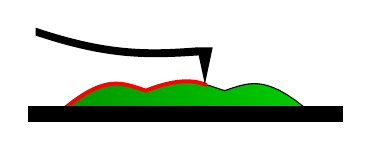
\begin{tikzpicture}
	% campione
	\shadedraw[left color=OliveGreen, right color=green!80!black] (0.5,0)
		.. controls (1, 0.4) and (1.2, 0.3) .. (1.5,0.2)
		.. controls (2,0.4) and (2.2,0.3) .. (2.5,0.2)
		.. controls (2.8, 0.3) and (3, 0.4) .. (3.5,0);
	%solco
	\draw[red, line width=0.5mm, line cap=rect] (0.5,0)
		.. controls (1, 0.4) and (1.2, 0.3) .. (1.5,0.2)
		.. controls (2,0.4) and (2.2,0.29) .. (2.25,0.28);
	%punta
	\fill (2.15,0.75) -- (2.25,0.28) -- (2.35,0.75);
	\fill (2.15,0.75)
		.. controls (1.5,0.7) and (1,0.7) .. (0.1, 1)
		-- (0.1, 0.9)
		.. controls (1,0.6) and (1.5,0.6) .. (2.2,0.65);
	%base
	\fill (0,0) rectangle (4,-0.2);
	\end{tikzpicture}
	\subcaption{Contatto}
	\end{subfigure}
	\begin{subfigure}{0.32\linewidth}
	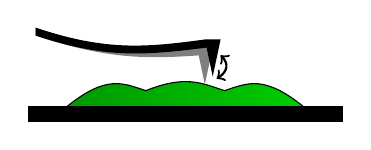
\begin{tikzpicture}
	% campione
	\shadedraw[left color=OliveGreen, right color=green!80!black] (0.5,0)
		.. controls (1, 0.4) and (1.2, 0.3) .. (1.5,0.2)
		.. controls (2,0.4) and (2.2,0.3) .. (2.5,0.2)
		.. controls (2.8, 0.3) and (3, 0.4) .. (3.5,0);
	%punta
	\fill[gray] (2.15,0.75) -- (2.25,0.28) -- (2.35,0.75);
	\fill[gray] (2.15,0.75)
		.. controls (1.5,0.7) and (1,0.7) .. (0.1, 1)
		-- (0.1, 0.9)
		.. controls (1,0.6) and (1.5,0.6) .. (2.2,0.65);
	%punta
	\fill (2.25,0.85) -- (2.35,0.38) -- (2.45,0.85);
	\fill (2.25,0.85)
		.. controls (1.5,0.75) and (1,0.7) .. (0.1, 1)
		-- (0.1, 0.9)
		.. controls (1,0.6) and (1.5,0.65) .. (2.3,0.75);
	%movimento
	\draw[<->, thick] (2.45,0.65) .. controls (2.55,0.55) and (2.55,0.45) .. (2.4,0.35);
	%base
	\fill (0,0) rectangle (4,-0.2);
	\end{tikzpicture}
	\subcaption{Contatto intermittente}
	\end{subfigure}
	\begin{subfigure}{0.32\linewidth}
	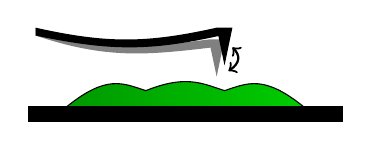
\begin{tikzpicture}
	% campione
	\shadedraw[left color=OliveGreen, right color=green!80!black] (0.5,0)
		.. controls (1, 0.4) and (1.2, 0.3) .. (1.5,0.2)
		.. controls (2,0.4) and (2.2,0.3) .. (2.5,0.2)
		.. controls (2.8, 0.3) and (3, 0.4) .. (3.5,0);
	%punta
	\fill[gray] (2.3,0.85) -- (2.4,0.38) -- (2.5,0.85);
	\fill[gray] (2.3,0.85)
		.. controls (1.5,0.75) and (1,0.7) .. (0.1, 1)
		-- (0.1, 0.9)
		.. controls (1,0.6) and (1.5,0.65) .. (2.35,0.75);
	%punta
	\fill (2.4,1) -- (2.5,0.52) -- (2.6,1);
	\fill (2.4,1)
		.. controls (1.5,0.8) and (1,0.8) .. (0.1, 1)
		-- (0.1, 0.9)
		.. controls (1.05,0.7) and (1.55,0.7) .. (2.45,0.9);
	%movimento
	\draw[<->, thick] (2.6,0.75) .. controls (2.7,0.65) and (2.7,0.55) .. (2.55,0.45);
	%base
	\fill (0,0) rectangle (4,-0.2);
	\end{tikzpicture}
	\subcaption{Senza contatto}
\end{subfigure}
\caption{Modalità di funzionamento di un microscopio \acrshort{afm}}
\label{fig:afm_modes}
\end{figure}

\subsection{Modalità a contatto} \label{s:afm_contact}

Nella modalità a contatto la forza normale, quindi l'inclinamento verticale del cantilever, è mantenuta costante durante la scansione. Quando la punta si sposta sopra una parte protrudente del campione, il cantilever viene spinto verso l'alto e si crea un errore sull'inclinazione verticale. Per correggere questo errore, il controllore alza la punta finché l'errore non si annulla. Quando si incontrano delle depressioni nel campione si opera il procedimento opposto, abbassando la punta.

Questa modalità permette anche di misurare le forze di attrito tra la superficie del campione e la punta ma non è utilizzabile su campioni biologici perché troppo delicati. La forza esercitata dalla punta può provocare stimoli meccanici non sostenibili per delle cellule e deformare biomolecole.\cite{zhong_1993}

Idealmente, la forza dovrebbe essere minore di 100pN per essere utilizzabile su biomolecole e nell'ordine dei nN per le cellule. Per questo motivo, vengono usati dei cantilever con una bassa costante elastica per diminuire il rumore, aumentare la sensibilità e diminuire la forza di interazione.\cite{wang_2018}

Un altro problema dell'uso di modalità a contatto è la possibilità che cellule poco aderenti o particelle di sporco si attacchino al cantilever.

\subsection{Modalità a contatto intermittente} \label{s:afm_ic}

Nella modalità a contatto intermittente, il cantilever oscilla verticalmente alla sua frequenza di risonanza, o poco meno. Quando la punta scansiona il campione, la sua altezza diminuisce l'ampiezza delle oscillazioni del cantilever che vengono misurate dal fotodiodo. Il segnale di controllo viene regolato in modo che, nel punto più basso del ciclo di oscillazione, la punta tocchi appena il campione. L'ampiezza di queste oscillazioni è quindi una misura delle interazioni tra la punta e il campione. Muovere la punta in alto e in basso, im modo da mantenere la stessa ampiezza di oscillazione, permette di ottenere una topografia del campione.

Altre informazioni ottenute da questo metodo sono l'ampiezza e fase dell'errore tra l'oscillazione del cantilever e il segnale di riferimento. Questo scostamento dal segnale pilota è causato dalla dissipazione di energia tra la punta e il campione, che può essere causato da delle deformazioni della superficie del campione o da forze di attrazione. Queste informazioni possono essere usate per ottenere proprietà viscoelastiche del campione e distinguere materiali diversi.\cite{bruker_phase_imaging}

Al contrario della modalità a contatto, la foza laterale è trascurabile visto che la punta tocca il campione solo per un istante ed è maggiormente indicata per campioni biologici, che altrimenti si muoverebbero liberamente insieme alla punta.\cite{karrasch_1993}

Questa modalità di operazione è più lenta rispetto alla modalità a contatto a causa del meccanismo di scansione. Mentre nella modalità a contatto intermittente il segnale è generato dalla modulazione in ampiezza del cantilever, nella modalità a contatto si usa la deflessione del cantilever, che varia molto più velocemente. Questa differenza si riflette anche nel comportamento del controllore: la modalità a contatto è più stabile ad alti guadagni, che invece possono generare forti artefatti o immagini rumorose nella modalità a contatto intermittente. I parametri del controllore devono quindi essere scelti con più attenzione. 

\subsection{Modalità senza contatto} \label{s:afm_nc}

Nella modalità senza contatto, la punta non tocca mai il campione ma mantiene comunque un'alta sensibilità alla sua topologia. Per fare ciò, la punta deve trovarsi abbastanza vicino al campione da entrare nel suo campo di forze, ma senza passare nella regione attrattiva usata per le modalità a contatto, quindi la scansione con questa modalità è eseguita esclusivamente nella regione attrattiva.

Questa scelta comporta l'uso di un cantilever molto rigido e farlo rimanere molto vicino alla superficie del campione per osservare come cambiano l'ampiezza e la fase della sua oscillazione, evitando che salti nel regime repulsivo. Questi sono effetti della variazione della frequenza di oscillazione in risposta alle forze applicate dalla superficie sulla punta (forze di van der Waals).

Per questa modalità si usa un cantilever ad alta frequenza di risonanza, tipicamente compresa tra 300 e 400 kHz, e bassa ampiezza di oscillazione, di circa 10nm.\cite{giessibil_1999} Come per la modalità a contatto intermittente, la velocità di scansione è più bassa di quella della modalità a contatto, ma queste proprietà del cantilever permettono di avere velocità maggiori della modalità a contatto intermittente.

Non entrando mai nella regione ripulsiva, questa modalità presenta il più basso rischio di danneggiare o contaminare la punta e il campione.\cite{ho_1996}

\vspace{2mm}

\begin{figure}[h]
\centering
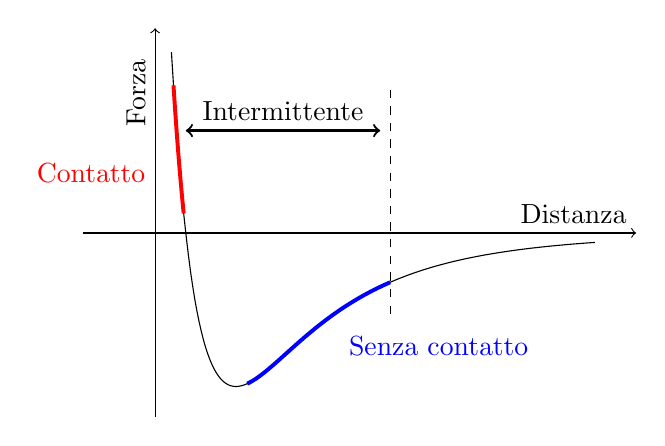
\begin{tikzpicture}[domain=1.93:4, samples=200, scale=2.6]
	%assi
	\draw[->] (1.5,0) -- (4.2,0) node[above left] {Distanza};
	\draw[->] (1.85,-0.9) -- (1.85,1) 
		node[above right,midway,sloped, xshift=11mm] {Forza};
		
	%grafico
	\draw plot (\x,{3*((2/\x)^(12)-(2/\x)^6)});
	
	%regione contatto
	\draw[domain=1.94:1.99, red, line width=0.5mm] plot (\x,{3*((2/\x)^(12)-(2/\x)^6)});
	\node[red,above left] at (1.85,0.2) {Contatto};
	
	%regione senza contatto
	\draw[domain=2.3:3, blue, line width=0.5mm] plot (\x,{3*((2/\x)^(12)-(2/\x)^6)});
	\node[blue,right] at (2.75,-0.55) {Senza contatto};
	
	%regione intermittente
	\draw[dashed] (3,0.7) -- (3,-0.4);
	\draw[<->, thick] (2, 0.5) -- (2.95,0.5)
		node[above,midway] {Intermittente};
\end{tikzpicture}
\caption[Grafico delle forze di van der Waals secondo il modello di Lennard-Jones] {
	\begin{tabular}[t]{ @{} l @{} }
		Grafico delle forze di van der Waals secondo il modello di Lennard-Jones\\
		Semipiano superiore: Forze repulsive\\
		Semipiano inferiore: Forze attrattive
	\end{tabular}}
\label{fig:waals}
\end{figure}

\subsection{Modulazione in frequenza}

Le modalità descritte nei paragrafi precedenti fanno tipicamente uso della modulazione in ampiezza. L'uso della modulazione in frequenza è limitato in quanto richiede attrezzature specifiche e un ambiente a vuoto ultra spinto. Usare una modalità oscillante a modulazione in frequenza ha anche dei vantaggi, come una vera risoluzione atomica.\cite{sugawara_1995}


\subsection{Sistema di controllo}

Il controllo del sistema è affidato a un controllore \acrshort{pid}, di gran lunga il tipo di sistema di controllo più usato (il 95\% di tutti i problemi di controllo si possono risolvere con questo sistema).\cite{astrom_2010}

\begin{figure}[h]
\centering
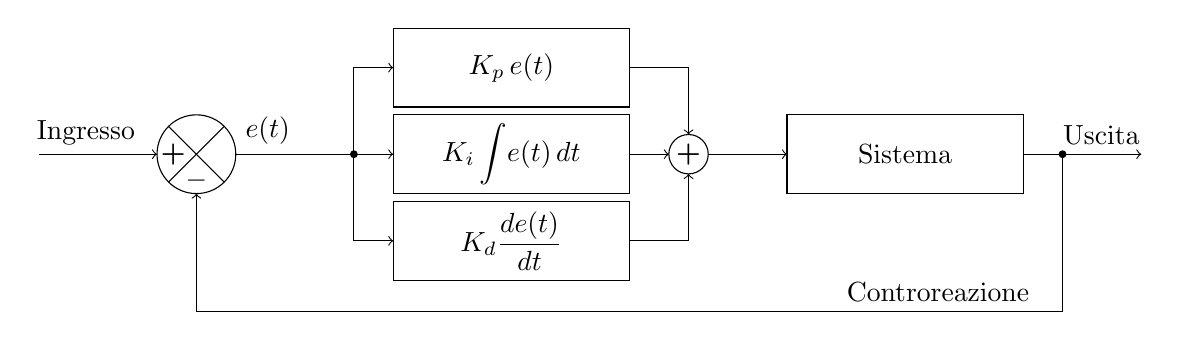
\begin{tikzpicture}
	
	\draw[->] (-2,0) node[above right, xshift=-1.5mm] {Ingresso} 
		-- (-0.5,0) node[right, xshift=-0.75mm] {\textbf{+}};
	
	\draw (0,0) circle (0.5);
	\draw (0.3535,-0.3535) -- (-0.3535,0.3535);
	\draw (-0.3535,-0.3535) -- (0.3535,0.3535);
	
	\draw[->] (0.5,0) node[above right] {$e(t)$} -- (2.5,0);
	\draw[->] (2,0) -- (2,1.1) -- (2.5,1.1);
	\draw[->] (2,0) -- (2,-1.1) -- (2.5,-1.1);
	\fill (2,0) circle (0.05);
	
	\draw[->] (5.5,0) -- (6,0);
	\draw[->] (5.5,1.1) -- (6.25,1.1) -- (6.25,0.25);
	\draw[->] (5.5,-1.1) -- (6.25,-1.1) -- (6.25,-0.25);
	\draw (6.25,0) circle (0.25) node {\textbf{+}};
	
	%controllore
	\draw (2.5,1.6) rectangle (5.5,0.6)
		node[midway] {$\displaystyle K_p\,e(t)$};
	\draw (2.5,0.5) rectangle (5.5,-0.5)
		node[midway] {$\displaystyle K_i\int\!e(t)\,dt$};
	\draw (2.5,-0.6) rectangle (5.5,-1.6)
		node[midway] {$\displaystyle K_d\frac{de(t)}{dt}$};
	
	\draw[->] (6.5,0) -- (7.5,0);
	\draw (7.5,0.5) rectangle (10.5,-0.5)
		node[midway] {Sistema};
	
	\draw[->] (10.5,0) -- (12,0) node[above left, xshift=1mm] {Uscita};
	\draw[->] (11,0) -- (11,-2) node[above left, xshift=-3mm] {Controreazione}
		-- (0,-2) -- (0,-0.5) node[above, yshift=-0.75mm] {$-$};
	\fill (11,0) circle (0.05);
\end{tikzpicture}
\caption[Diagramma di un controllore PID ad anello chiuso] {
	\begin{tabular}[t]{ @{} l @{} }
		Diagramma di un controllore PID ad anello chiuso\\
		$e(t)$: funzione di errore
	\end{tabular}}
\label{fig:pid_diag}
\end{figure}

Quando le forze di interazione tra la punta e il campione cambiano, il cantilever si flette e, di conseguenza, modifica l'uscita del fotodiodo facendola deviare dal valore di ingresso. La differenza tra ingresso e uscita è la funzione di errore $e(t)$.

Il controllore PID agisce su questa funzione e il suo comportamento è composto da tre azioni indipendenti, controllate da altrettante variabili di regolazione.\cite{ogata_2010}
\begin{itemize}
	\item Il termine \textbf{P} (\textit{azione proporzionale}) è proporzionale alla funzione di errore
	\item Il termine \textbf{I} (\textit{azione integrativa}) è l'integrale dei valori passati di $e(t)$
	\item Il termine \textbf{D} (\textit{azione derivativa}) è una stima delle variazioni future di $e(t)$
\end{itemize}

Il sistema di feedback comprende tre meccanismi principali:
\begin{enumerate}
	\item Il tubo piezoelettrico per il controllo del movimento e della posizione della punta rispetto alla superficie del campione
	\item Il cantilever e il sistema ottico per la misura della distanza tra la sonda e la superficie del campione
	\item Il circuito di controllo per mantenere una deflessione costante correggendo la tensione applicata al tubo piezoelettrico
\end{enumerate}

\subsection{Parametri del sistema}

Per sua natura, un microscopio \acrshort{afm} è molto versatile e presenta molti parametri che si possono regolare per ottimizzare la resa delle immagini. Partendo da quelli più generali, si può impostare una modalità operativa, come quelle descritte sopra (\textit{vedi} \ref{s:afm_contact}, \ref{s:afm_ic}, \ref{s:afm_nc}), e un tipo di cantilever che più si adattano al campione scelto.

Passando ai parametri di scansione, si possono impostare la velocità e l'area di scansione controllando opportunamente il sistema piezoelettrico su cui poggia il campione. L'area di scansione rappresenta il campo di osservazione del campione (es. 10 µm × 10 µm) ed influenza la risoluzione delle immagini. La velocità di scansione, espressa in µm/s o linee al secondo (Hz), è inversamente proporzionale alla qualità dell'immagine, ma con basse velocità aumenta il rischio di muovere parti del campione.

È possile anche regolare dei parametri relativi all'interazione tra la punta e il campione, come l'ampiezza e la frequenza di oscillazione (solo in modalità oscillanti) e la forza di carico desiderata. Per regolare questi parametri si può operare sull'ingresso del sistema e sul guadagno dell'anello di feedback.

\section{SNOM}

\section{Batteri}

\end{document}
